\chapter{Fundamentals}
\label{chap2}

\section{Glance}

As described in the previous chapter, Glance \cite{grael-tcc} \cite{maidantchik-glance} was a technology built in 2003, during the construction phase of the ATLAS experiment, by former UFRJ students to meet custom CERN needs. As Felipe Grael, its original author, describes, Glance was a generic web system for retrieving an extensive amount of data from multiple databases from the ATLAS experiment \cite{grael-tcc}. It was developed mostly in C++, successfully achieving the goal of centralising access to collaboration data, being accessible anywhere to all collaborators, and facilitating users to create search interfaces without any programming skills or knowledge of the database structure.


\section{FENCE}

In 2013, the Glance Team developed the Frontend Engine for Glance (FENCE) \cite{lange-tcc}. As the name states, it was a framework built to generate user interfaces that could read data from Glance, removing the responsibility of the previous system to deal with presentation layers and focusing on search interfaces.

One of FENCE's main goals was to share features between applications. It provides an object-oriented ecosystem written in PHP that allows code reuse by defining abstract classes with base functionalities. FENCE dependents could then extend the classes by overriding the desired methods in order to implement custom functionalities.

The inheritance characteristic is exemplified \autoref{fig:fence-inheritance}. FENCE defines an abstract \texttt{Content} class to display content to the end user. It also implements a \texttt{BaseProfile}, extending \texttt{Content} and adding features to be used on profile pages among FENCE dependents. The ALICE Membership application depends on FENCE and has a member profile page represented by the \texttt{Profile} class, which extends the \texttt{BaseProfile} inheriting behaviour from \texttt{BaseProfile}, \texttt{Content} and adding custom functionalities like the ones on the \texttt{post()} method.

\begin{figure}[htbp]
  \centering
  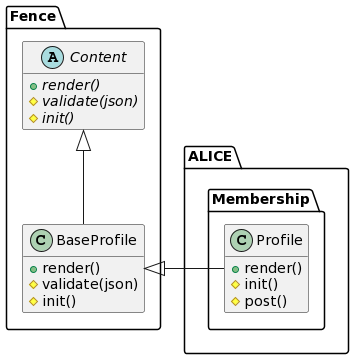
\includegraphics[scale=0.7]{Imagens/chap02/fence-class-diagram.png}
  \caption{Inheritance between FENCE and ALICE Membership classes.}
  \label{fig:fence-inheritance}
\end{figure}

The code block on \autoref{code:fence-usage} illustrates how applications use FENCE. Every page shares a skeleton composed of importing dependencies (line 5), FENCE initialisation (line 8), content injection (line 10), rendering (line 12) and error handling (lines 13 and 14).

\begin{listing}
\begin{minted}{php}
<?php

use Fence\Fence;

require_once "autoload.php";

try {
    $fence = new Fence();
    
    $fence->add_menu("menu.json");
    
    $fence->render();
} catch (Exception $exception) {
    Fence::handle_exception($exception);
}
\end{minted}
\caption{FENCE usage example.}
\label{code:fence-usage}
\end{listing}

Once a page request arrives at the server, FENCE is initialised. A single command for the application developer unleashes multiple setups behind the scenes. The logger is initialised. Error handling is configured, writing the message into a log file and sending emails in case of fatal errors. JSON configuration files are parsed, and the configuration is set. A new connection to the application database is opened. The user is authorised. Database connection and user details are made available globally through the application. The page layout, header and footer are added to the HTML response. JavaScript and CSS files are loaded, including third-party libraries and injected into the response.

Next, the application adds content to the page response. In this example, a menu is added by providing the path of a JSON configuration file with all the desired titles, labels and links from the menu. FENCE also supports adding complex search interfaces, forms, profile pages and other custom content.

The \texttt{render} method outputs the complete HTML, sending it via an HTTP response to the end user browser to display the application's page. Finally, any unhandled exception is caught and handled by logging the message into the user's log file, emailing the responsible developers, and displaying a user-friendly error page.

\section{Drawbacks of an in-house framework}

At least twenty systems were developed using FENCE \cite{pinhao-tcc} and are part of the tools used by collaborators from the ATLAS, ALICE and LHCb experiments. The framework allowed the Glance Team to rapidly create new applications by exposing common features as abstract classes and adding custom behaviours via configuration files. However, after years of dealing with it, the developer team realised and agreed that the framework and its design were responsible for the high maintenance cost of the systems, resulting in little time to develop new applications \cite{de-jesus-tcc}. The limitations of FENCE are part of the motivation for this work and will be examined in more detail in the next subsections. 

\subsection{Installation}

The dependencies requirements of FENCE systems were not well defined and dispersed. For example, the framework itself was referenced in a combination of Composer (a PHP package manager \cite{composer-website}) import and an Apache configuration. Third-party libraries and installation scripts were defined on multiple package managers and task runner tools such as Composer, npm \cite{npm-website}, Bower \cite{bower-website} and Grunt\cite{grunt-website}. Application configurations were also split in FENCE's \texttt{configuration.json}, Apache and PHP configuration files, each in separate directories on the file system and not available on the version control system.

FENCE needed to be better decoupled from the database, being highly dependent on a connection to specific Oracle databases with access to CERN's Human Resources data. Together with the characteristics described in the previous paragraph, applications built with the framework were generally hard to install. Glance Team members had to develop the applications on CERN servers since the long list of dependencies and configurations took much work to replicate locally. Developing remotely was not ideal, especially for the Brazilian students part of the team, who had to depend on unstable SSH connections to computers in Switzerland, significantly increasing latency and development speed. 

Another issue brought about by the FENCE installation was the deployment to production. Since new features and bug fixes were deployed in chunks, it was common for developers to forget to include updated configurations during the deployment. Such mistakes often resulted in crashes and more bugs in production systems.

\subsection{Learning curve}

Due to the characteristics of the collaboration between students of UFRJ and CERN, the Glance Team has a high turnover of developers, with most of the members being replaced every two years by new ones, often on their first work experience. It is then necessary for the applications to provide a low learning curve for the new group, meaning that they should learn fast and have enough time to contribute by creating new systems and features \cite{de-jesus-tcc}.

Learning FENCE, however, was slow. The lack of documentation allied with hidden coupling on the framework were a bottleneck on the first step of learning FENCE. The alternative options were to learn by studying examples of existing systems and asking senior colleagues for guidance, which could have been more time-efficient. It took 6 to 12 months for new members to have intermediary knowledge of the framework and build significant contributions.

\subsection{Reinventing the wheel}

As a framework, FENCE was not only a front-end layer for Glance. It had other responsibilities, such as a logger, ORM, database connection interface, email messenger, error handler and configuration parser. The issue is that all those features were in-house solutions for known problems in the industry that had already been solved. At first, they seemed to have simple requirements but became a burden for the following developers who had to dedicate time to their maintenance.

The members of the Glance Team spend most of their time building applications for the experiments at CERN, with no member fully dedicated to the FENCE framework and its in-house solutions. On the other hand, open-source libraries have a team of dedicated developers with expertise in the problem domain, good documentation, and tests. They were battle-tested by thousands, if not millions, of other applications in the industry. By outsourcing some of its features, the team could decrease development costs, reduce the overall learning curve, and increase both framework and systems quality.

\subsection{Usage of global variables}
\label{sec:global-variables}

Applications built with FENCE access frequently used data such as current user, database connection and system configurations through global variables. The instances are set on the framework initialisation and available anywhere on the code base. At first, it appears to be an easy way to access commonly used objects, but this convenience has a price. Global variables can be modified in any part of the program, making it difficult for developers to reason about every place where it is used and ignore constraint checks. Other drawbacks with global variables include implicit coupling, concurrency issues, namespace pollution and problems with test setups \cite{rishikesh}.

\subsection{The FacTree ORM}

FacTree, an acronym for Factory Tree, is a micro-ORM (Object-Relational Mapping) built and used by FENCE applications to convert rows from the database into PHP objects. Following the framework's principles, entities were configured with JSON files, with definitions of property, constraints, and relations.

The primary issue with FacTree was the memory problems when retrieving multiple objects from the database. Entities with multiple relations made intensive memory usage, resulting in crashes on search results with more than 2000 objects due to memory overflow. From the final user perspective, this issue negatively impacted the usage of FENCE systems.

Other drawbacks of the in-house ORM include lacking support for basic operations besides reading and an incomplete filtering solution. Operations such as creating, updating and deleting entities were not supported and must be performed by executing SQL queries. The filter functionality only worked on the main properties of the object and was inconsistent on relation filters.

In an ideal environment, the issues listed could be solved with some effort from the developer team. However, the nature of FacTree, with most of its logic on a single file, the absence of tests and multiple dependents made changes on the ORM always critical.

\subsection{Lack of tests}

Some of the issues of FENCE usage could be solved if both the framework and its dependents had automated tests. Early testing brings to light multiple problems before deploying a program, such as architectural flaws, poor design decisions, incorrect functionality, security vulnerabilities and scalability issues \cite{ibm-software-testing}. Software without tests usually is not easily maintained. It is prone to accumulate technical debt since the impact of changes and new features is hard to predict as the system evolves.

In 2018, an effort was made to add tests to applications created by the Glance Team \cite{alves-tcc}. However, it was not trivial due to the design flaws of FENCE and the lack of isolation between the systems and the framework. As described in previous sections, FENCE classes were highly coupled with external resources such as database connection, configurations on the filesystem, user information from CERN Single Sign-On and HTML output. The coupling was the root cause for the difficulty in writing tests since it took considerable work to set up a test environment by mocking all the resources and not being able to verify the behaviour of the software in small units. The fact that applications were not isolated from FENCE resulted in the same dependency on resources and, therefore, struggle in writing tests.

\section{REST API}

Representational State Transfer (REST) is an architectural style for distributed hypermedia systems, introduced by Roy Fielding in 2000 \cite{fielding-rest}. A system and a Web API  conforming to the  REST architectural constraints are referred to as RESTful and REST API, respectively \cite{restfulapi-site}.

The first constraint proposed in REST uses a \textbf{client-server} architectural style, focusing on separating concerns between the user interface and data storage. The isolation of client and server benefits an independent evolution of the components, allowing the portability of the front end to multiple devices and the scalability of the back end according to organisational domains. Clients and servers may be written in different programming languages and follow distinguished paradigms but work together through an intermediary interface.

REST defines a \textbf{uniform interface} between clients and servers. A resource should be fetched in a single way and should not be too extensive, containing everything it represents, but should contain links to fetch related information. Specific guidelines should be followed throughout the system, such as read-and-write approaches, naming conventions and data format. Once a developer using the API learns how to manipulate one resource, it should be able to apply a similar approach to other parts of the interface.

One of the most common usages of REST is on Web APIs. Through HTTP, a client sends a request to a server with a combination of URL and HTTP method, referred to as endpoint or route. The server processes the request and returns a response with the result data, usually in a human and machine-readable format such as JSON or XML. There is intense usage of HTTP methods, headers, URI path and parameters, body, and status codes in the communication between the front and back ends.

\autoref{fig:rest-api} illustrates the messages exchanged between the server and two clients of a fictional bookstore API. To insert a book on the data store, Client 1 sends a \texttt{POST} HTTP request to the server with the URI of the \textit{book} resource and JSON data on the message body. The server processes the content of the message, inserts the book and returns an HTTP response with a 201 (Created) status code and a body with the identifier of the new book. Afterwards, Client 2, on another platform, fetches the same book information by sending a \texttt{GET} request with a URI containing the book ID and receives an OK response containing the book information.

\begin{figure}[htbp]
  \centering
  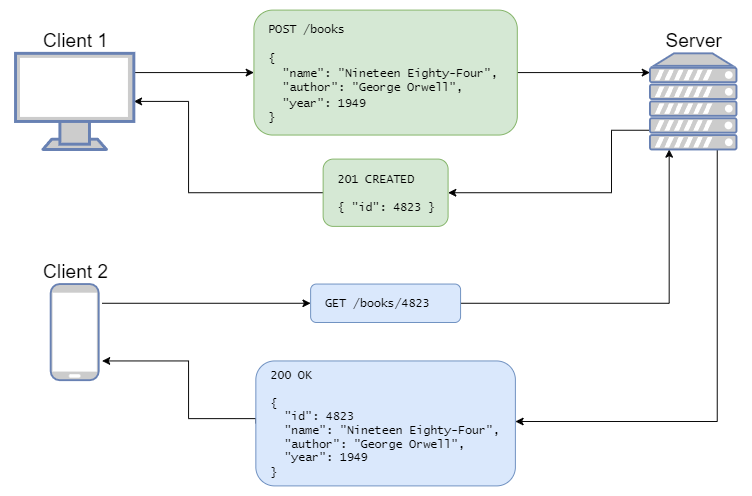
\includegraphics[scale=0.565]{Imagens/chap02/rest-api.png}
  \caption{Messages exchanged between clients and server on a fictional bookstore REST API.}
  \label{fig:rest-api}
\end{figure}

\section{Data exchange across CERN}

Software systems, including the ones developed by the Glance Team, are fundamental to the organisation of CERN experiments. Even with different scopes, the intersection of data between applications was not rare \cite{de-jesus-tcc}. For example, multiple systems depend on the Foundation Database \cite{foundation-website}, a centralised source of CERN's participants, hierarchical structure of organisation units, roles and addresses. Applications access Foundation's information by querying shared database views.

Besides consuming Foundation data, Glance applications communicate with other CERN systems by reading, writing and sharing information. Data sharing followed the same approach as Foundation: read access to the database was given to external services, which consumed information via tables and views. Glance-dependent components would need to connect to Glance's Oracle databases. Connecting to another database, however, is not always trivial. External systems may additionally have to install Oracle drivers, create accounts on the database or integrate their and Glance's databases directly. Changes in the original data source could cause side effects on dependent systems without notice. Finally, the sharing of personal information became critical after CERN started to comply with the General Data Protection Regulation (GDPR) \cite{gdpr} under Operational Circular no. 11 \cite{cern-operational-circular-11}.

In 2019, CERN Analysis Preservation (CAP) was interested in ATLAS Glance Analysis system data. CAP is a service for researchers to preserve and document the various components of their physics analyses by describing and structuring the knowledge behind an analysis to be understandable and reusable in the future \cite{cap-website}. Glance Analysis is the application that manages the analyses for the ATLAS experiment \cite{atlas-glance-analysis} \cite{pinhao-tcc}. CAP requested access to ATLAS Analysis data in an effort to centralise analysis information from all experiments. Knowing about the issues with direct database access, the external group asked the Glance Team if they could provide a REST API.

The request made by CAP was the starting point of this work. Glance Team started to study how to structure a REST API and make it available to other users and services. The developers quickly realised that the project was an excellent opportunity to start the segregation of the front and back end of Glance systems, with the user interface being one of the consumers of the new REST API.

\section{Service Work}

In order to ensure the full success of the ALICE experiment operation, a list of tasks is established and maintained. These tasks are also known as service work and concern detector maintenance, operation, calibration, quality control, data processing and outreach, coordination and managerial roles in the collaboration \cite{alice-collaboration-service-work}. The ALICE service work proposal was approved in August 2019 to be started in 2021 \cite{service-work-modus-operandi} and defines the share of work to be done by Member Institutes as described in the collaboration constitution \cite{alice-constitution}.

In order to manage the service work of ALICE, the Glance Team developed the Glance Service Work system \cite{alice-glance-sw-website}. It is a web application that handles task planning and assignments, accounting of work due and done by institutes, institute clusterisation and enforces rules to protect members of the collaboration of overwork.

Glance Service Work was developed in parallel with the work described in this document and was one of the first Glance Team systems with front and back ends decoupled using a REST API and without any dependency on the FENCE framework. It is a successful case of implementation of this project, being developed during all the evolution phases of this work. Due to this reason, its requirements and source code will be used as examples in the following chapters. From now on, the Glance Service Work system will be identified simply as Service Work.
